% !TeX spellcheck = en_US
% !TeX root = ../BachelorThesis.tex
\appendix
\numberwithin{figure}{section}
\chapter{Appendix}

\section{GPS Plots Straight Path}
%
\begin{figure}[H]
	\centering
	\subfloat[]{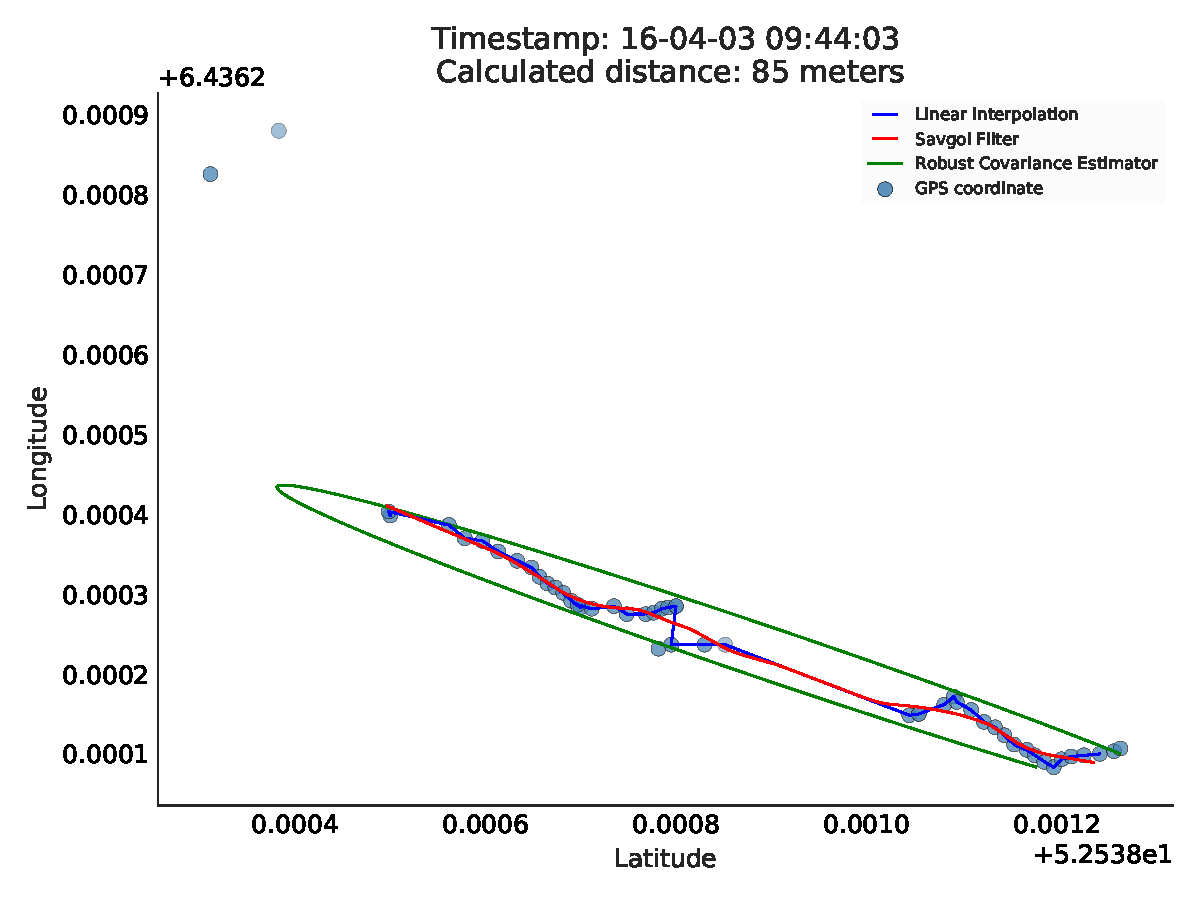
\includegraphics[scale=0.29]{gps/straight/3wAkwQDaLY7gYrhPi}
	}
	\hspace{0.5cm}
	\subfloat[]{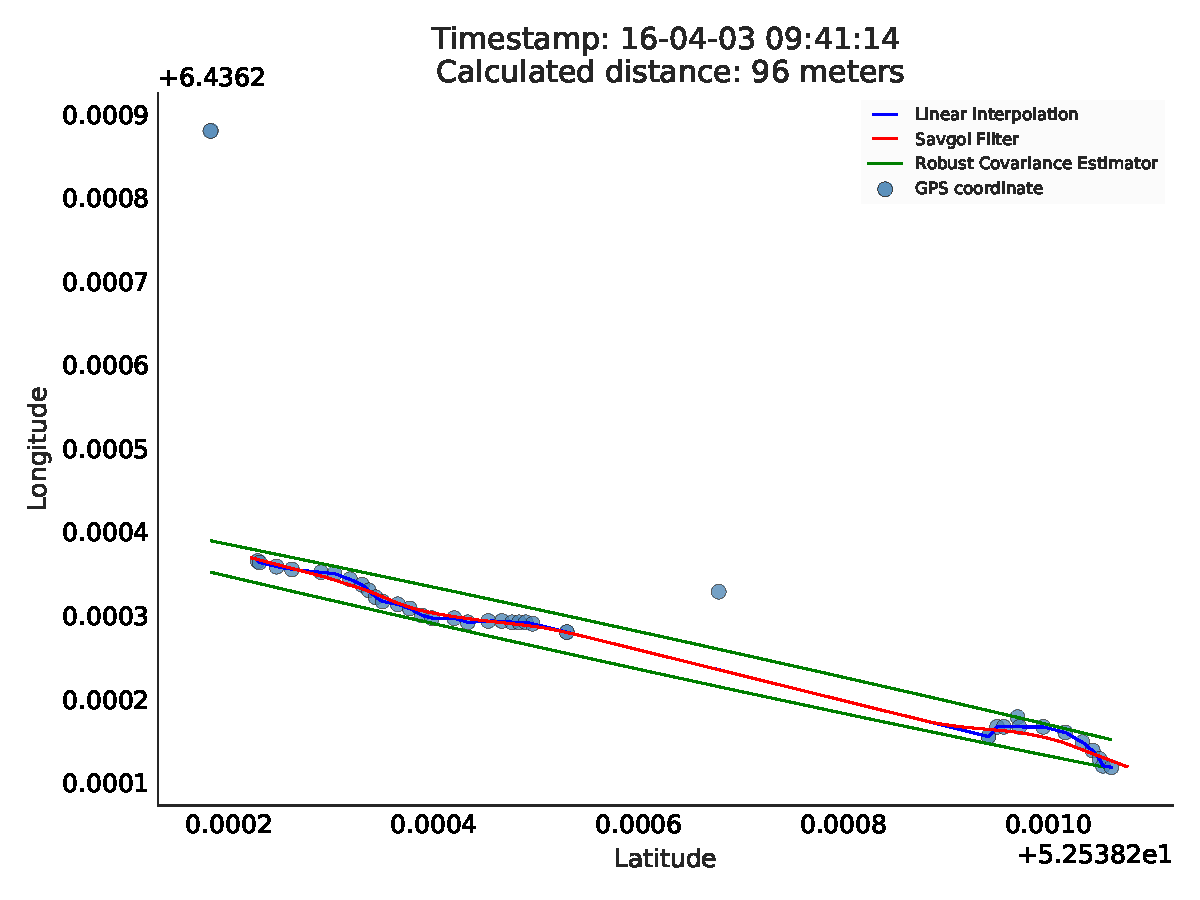
\includegraphics[scale=0.29]{gps/straight/9cuCTXcBBK2J32PoE}
	}
	\vfill
	\subfloat[]{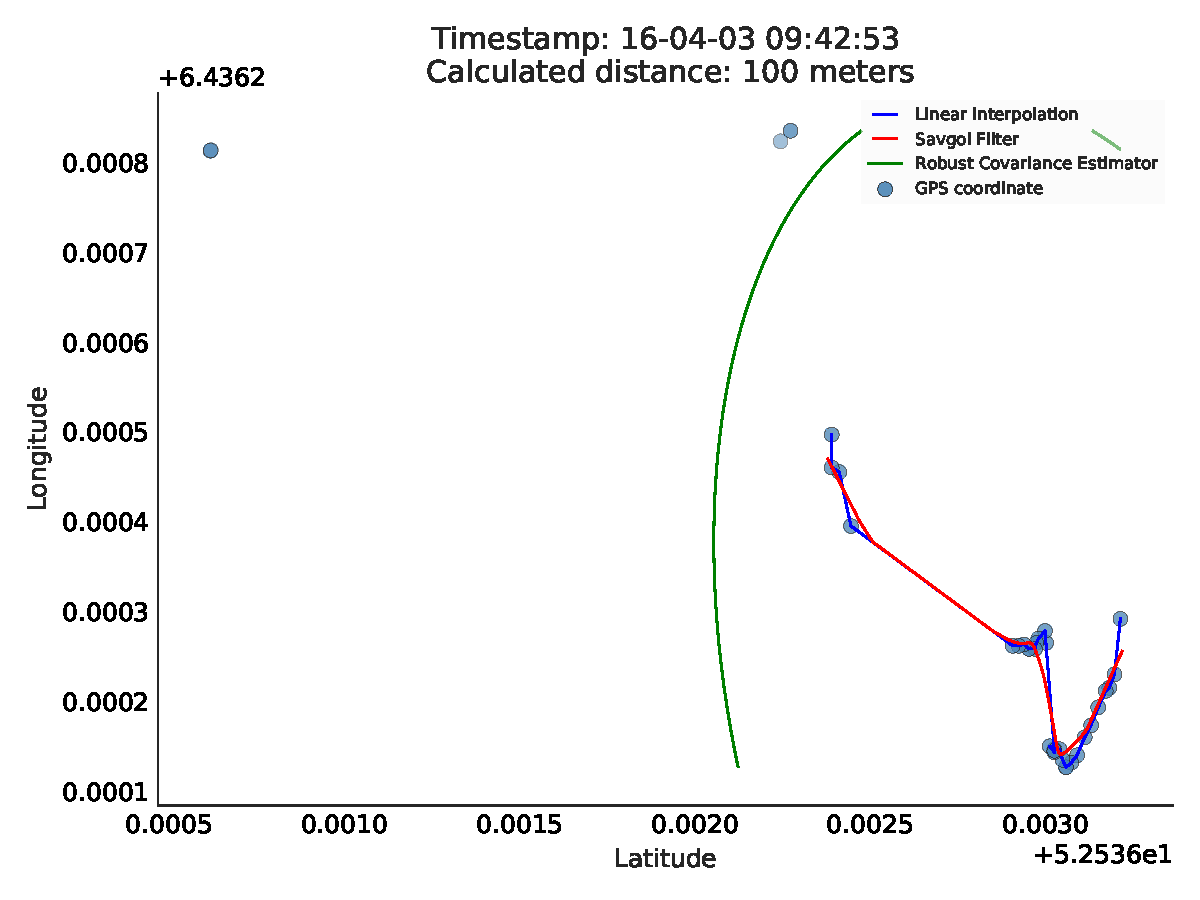
\includegraphics[scale=0.29]{gps/straight/Ba8aoCEfdhz2nxYq9}
	}
	\hspace{0.5cm}
	\subfloat[]{\label{fig:Terrible GPS Coordinates 1}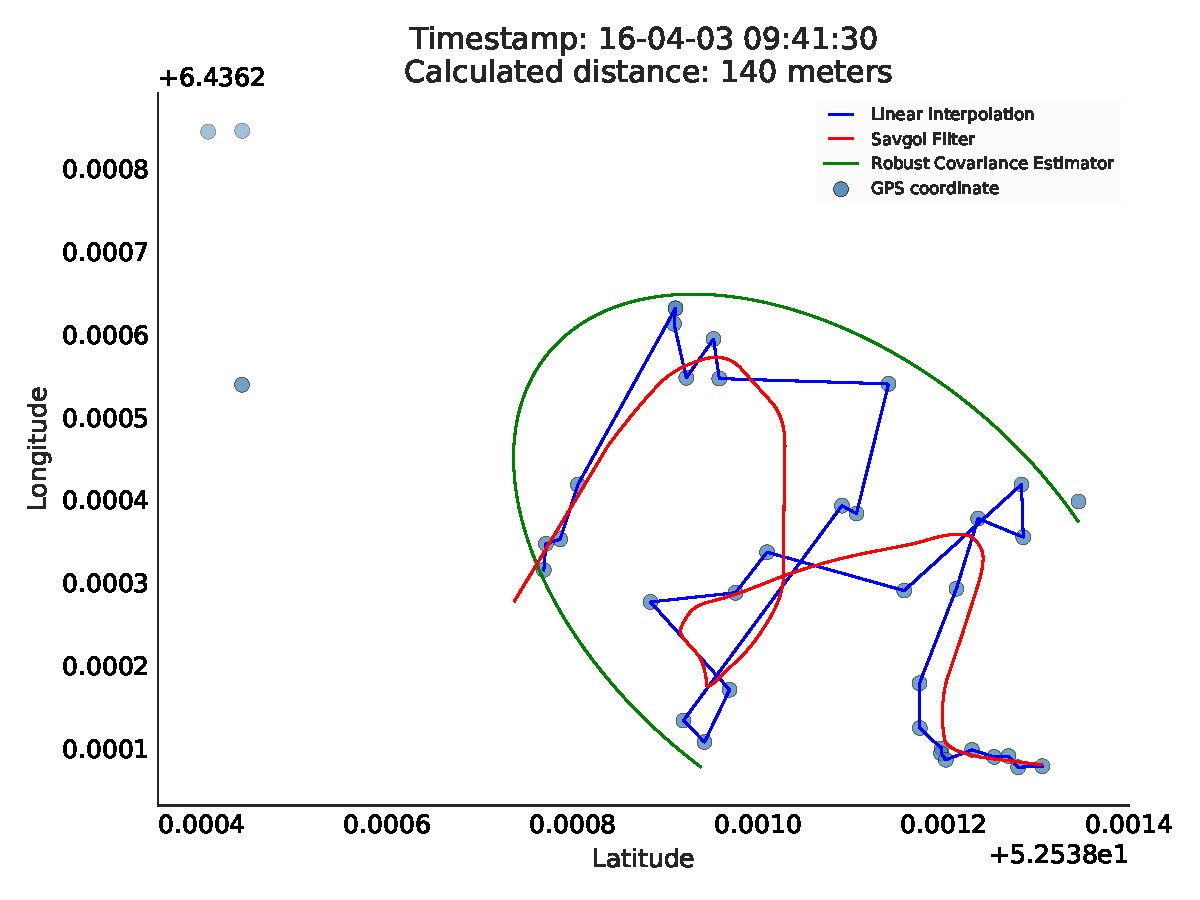
\includegraphics[scale=0.29]{gps/straight/CbpZDcgq8d6BCy5mj}
	}
	\captionof{figure}{Plots of the GPS coordinates of the walking test before and after smoothing. First, outlier detection is done using Elliptic Envelope. Afterwards, inliners are  smoothed in two stages: `Lineair Interpolation' is the first smoothing step and `Savgol Filter' the last.}
	\label{GPS Plots Straight Line}
\end{figure}
%
\begin{figure}[H]
	\ContinuedFloat 
	\centering
	\subfloat[]{\label{fig:Terrible GPS Coordinates 2}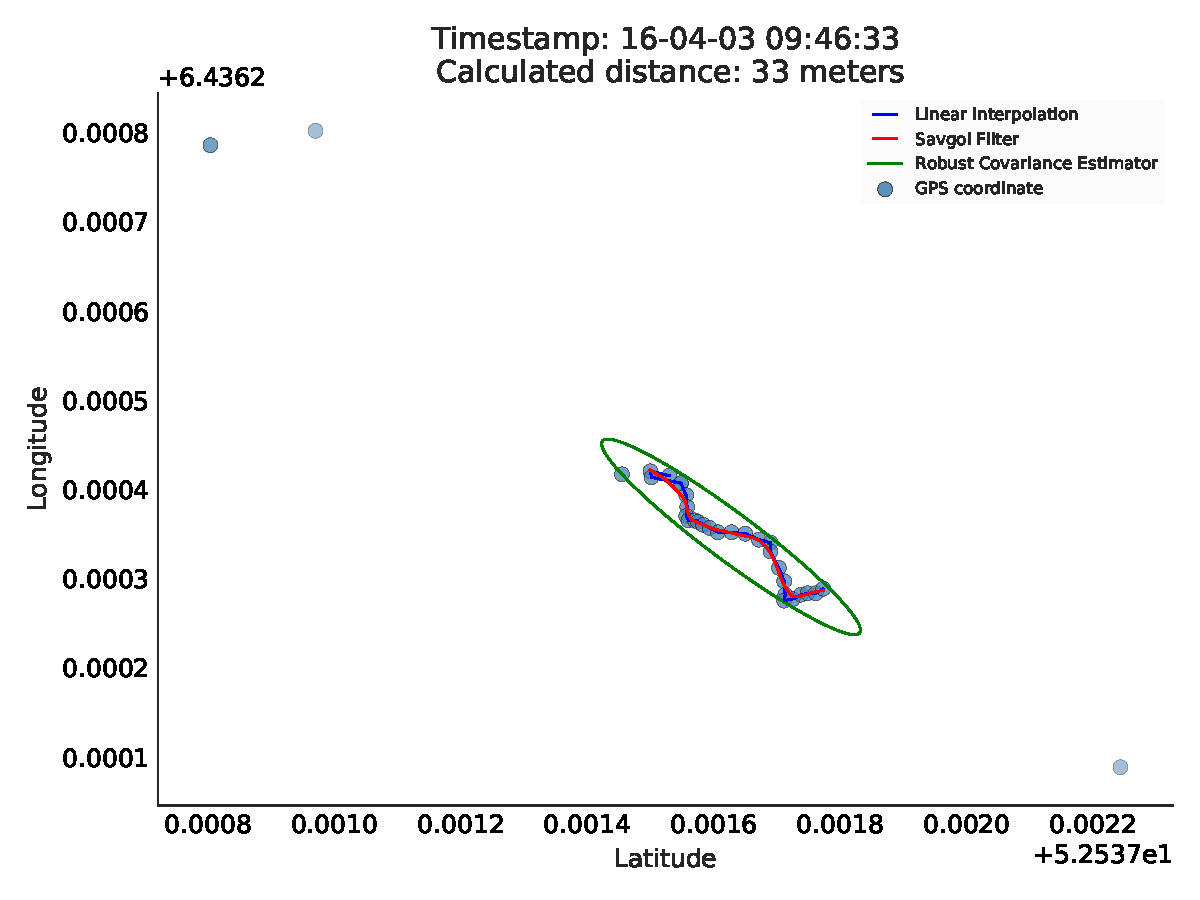
\includegraphics[scale=0.29]{gps/straight/exCkb4K2cCaZHHg4b}
	}
	\hspace{0.5cm}
	\subfloat[]{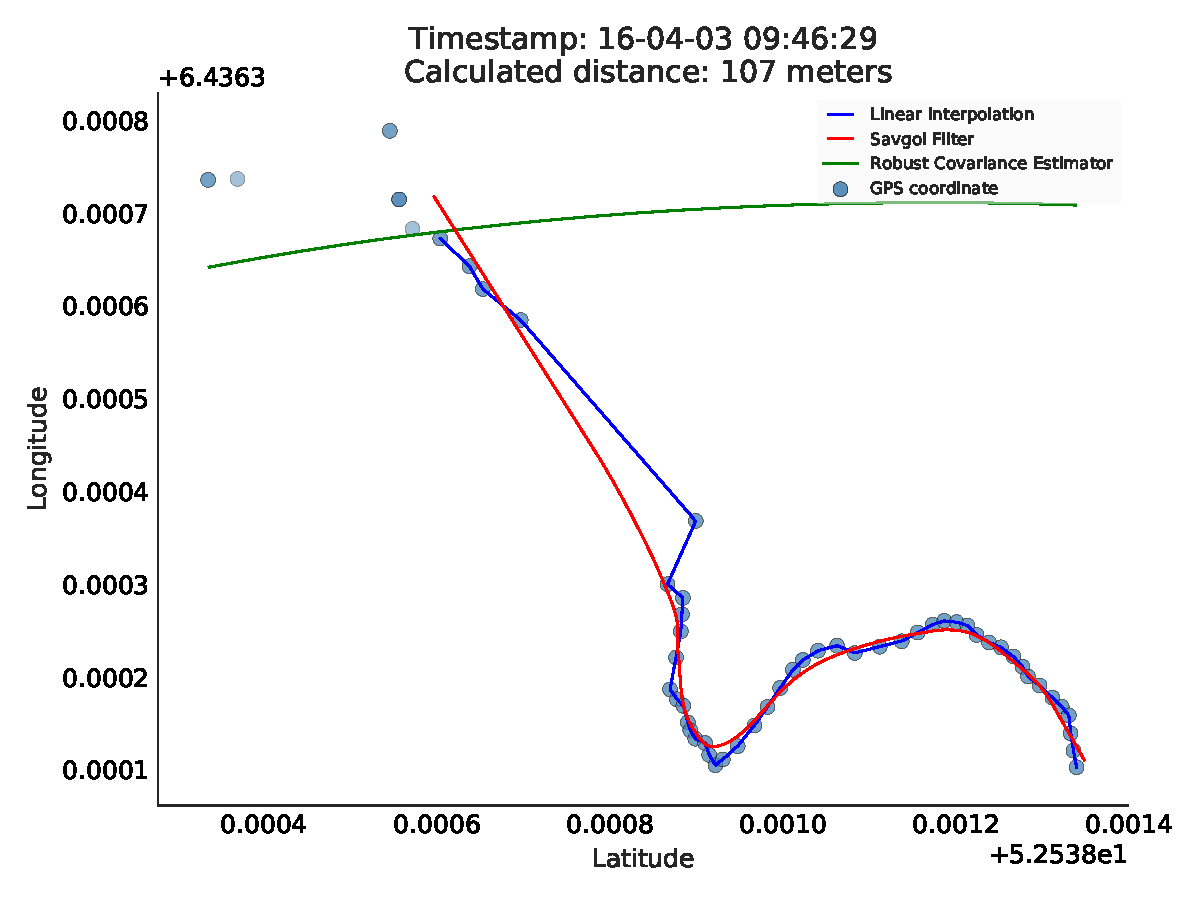
\includegraphics[scale=0.29]{gps/straight/fA2QJHC6iPcAmnu4x}
	}
	\vfill
	\subfloat[]{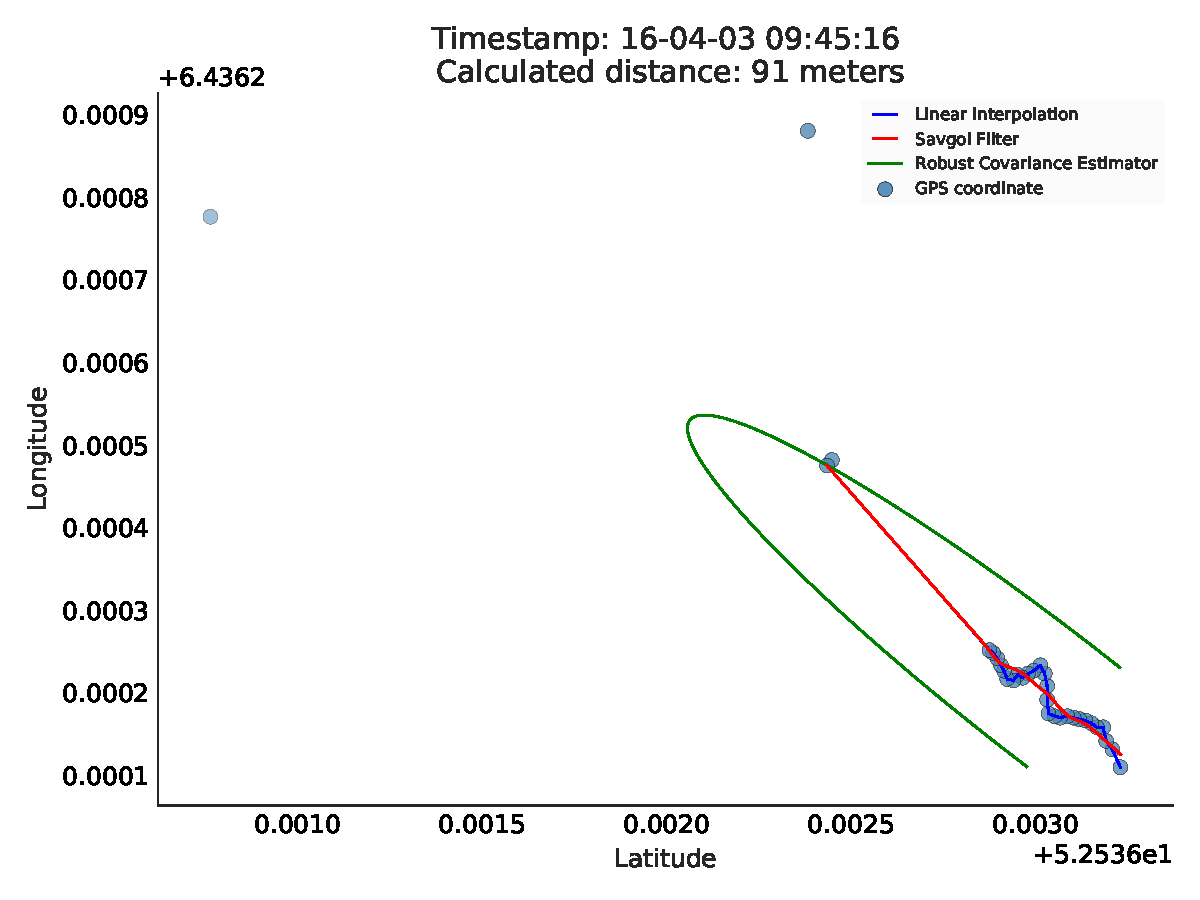
\includegraphics[scale=0.29]{gps/straight/g7zX6A4FnTu4L975N}
	}
	\hspace{0.5cm}
	\subfloat[]{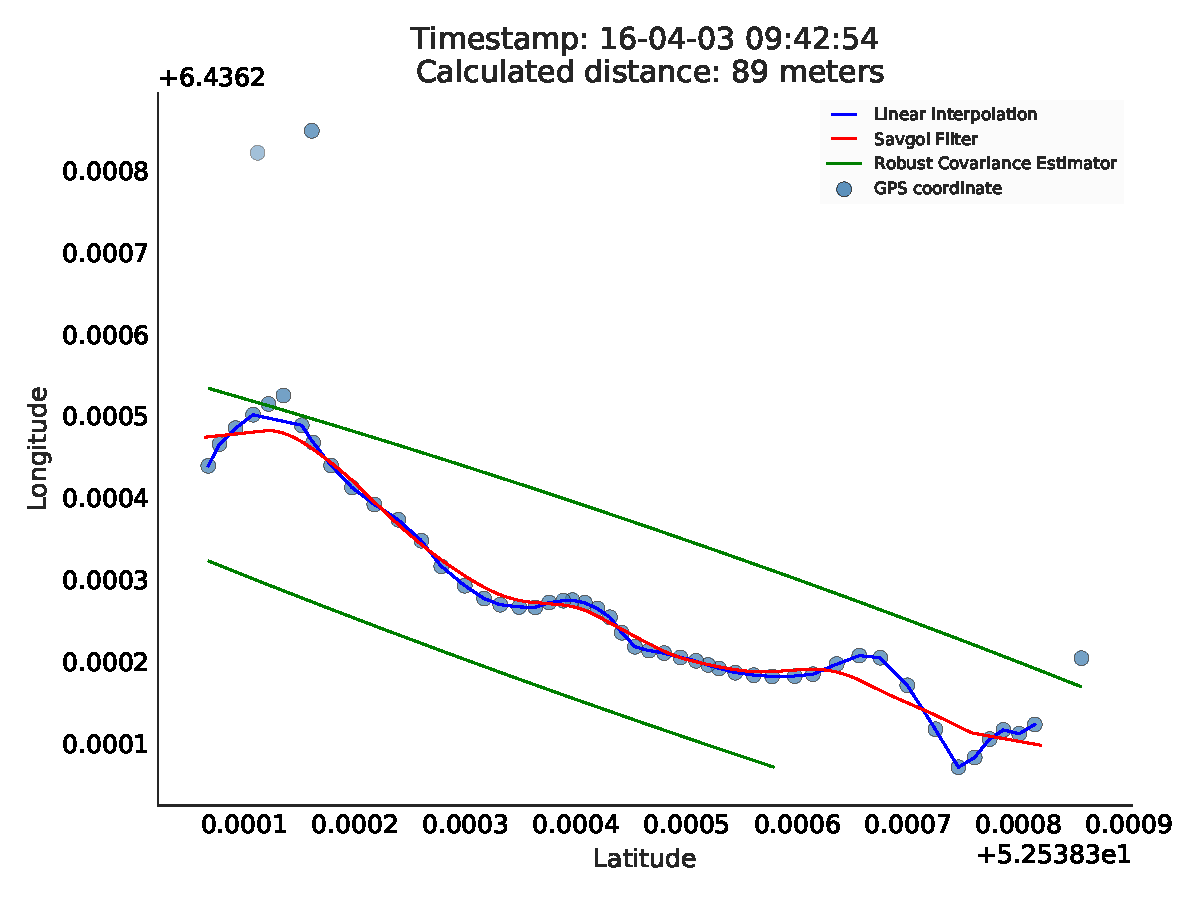
\includegraphics[scale=0.29]{gps/straight/KFb4FtR8Jjb6Ajtdc}
	}
	\vfill
	\subfloat[]{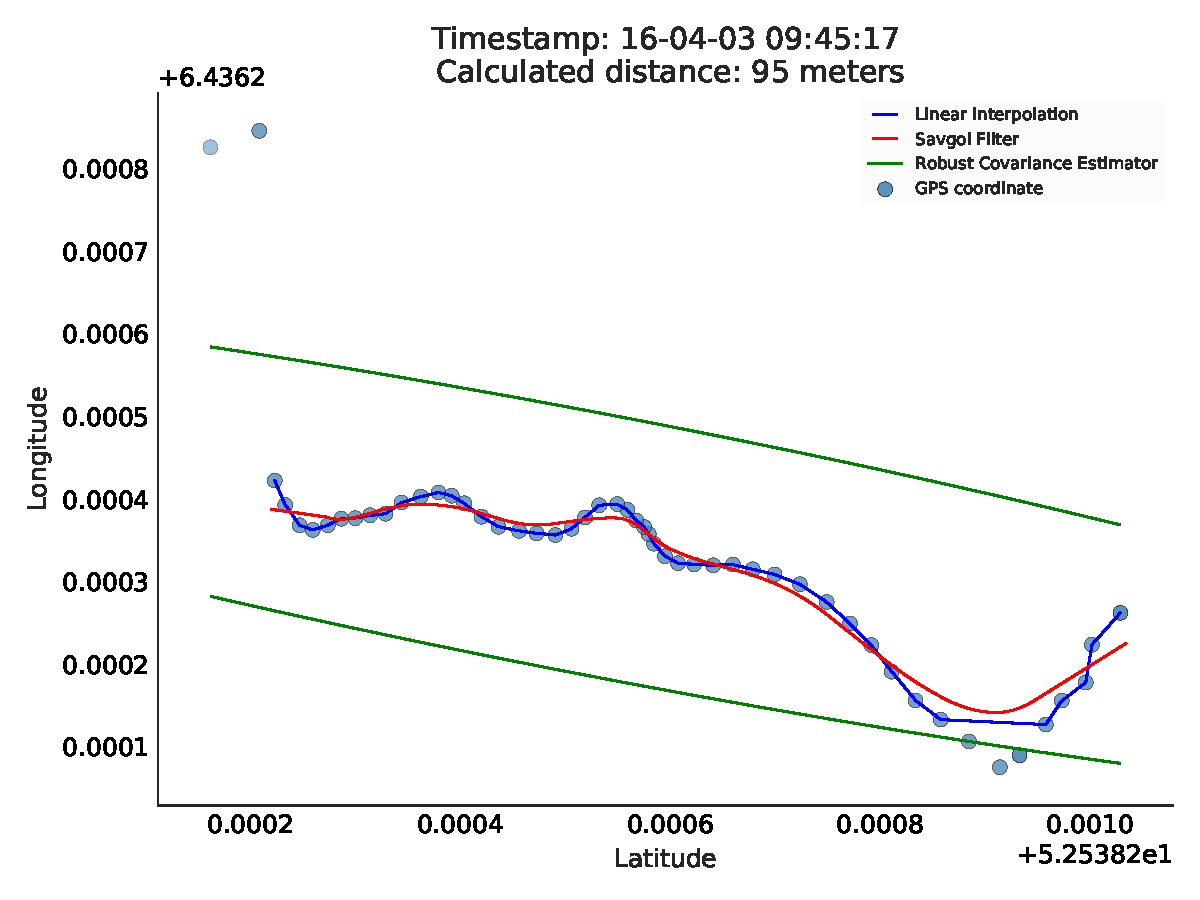
\includegraphics[scale=0.29]{gps/straight/QXtSsihbjmWnG854C}
	}
	\hspace{0.5cm}
	\subfloat[]{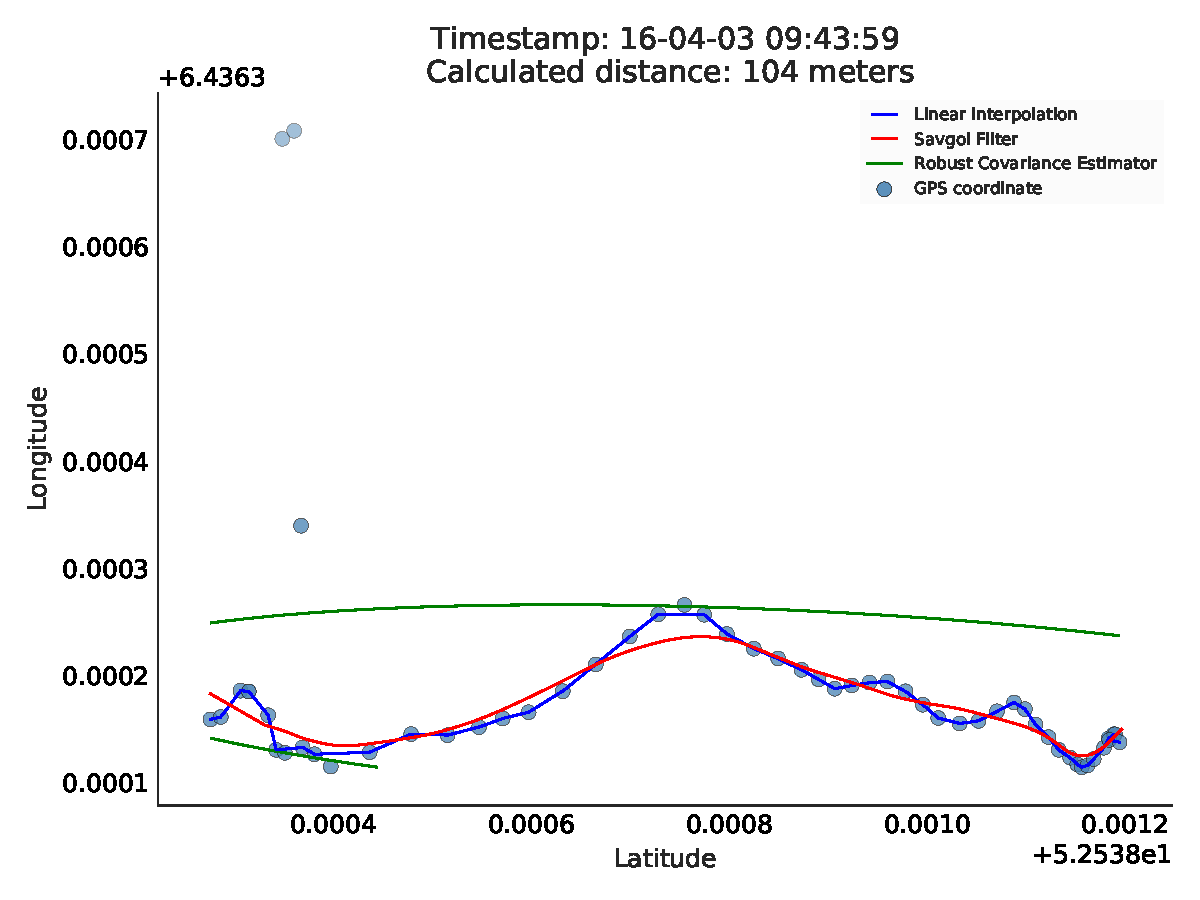
\includegraphics[scale=0.29]{gps/straight/vGn6KLTyNqBEH25YN}
	}
	\captionof{figure}{}
\end{figure}

\newpage

\section{GPS Plots Circular Path}
\begin{figure}[H]
	\centering
	\subfloat[]{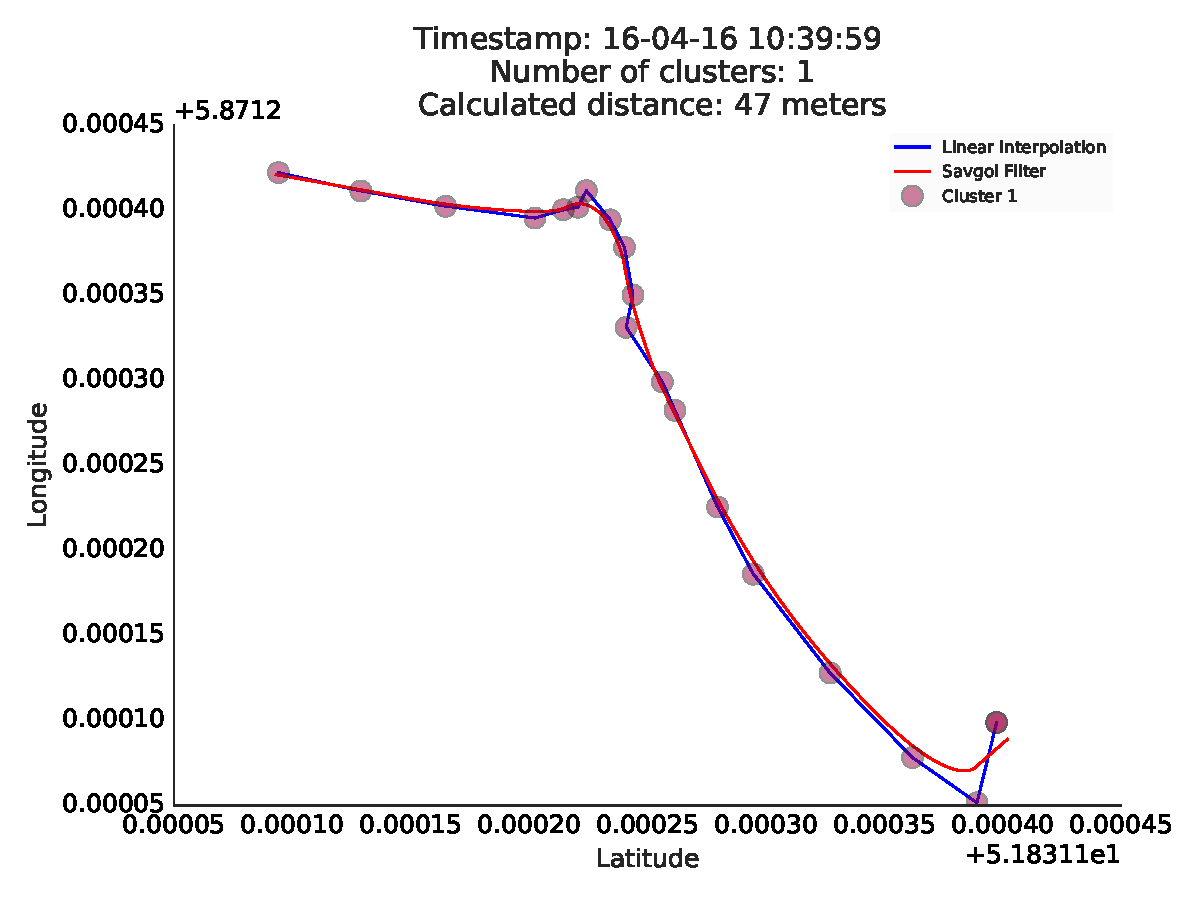
\includegraphics[scale=0.29]{gps/circle/2Zye5dTxYRNq7K7se}
	}
	\hspace{0.5cm}
	\subfloat[]{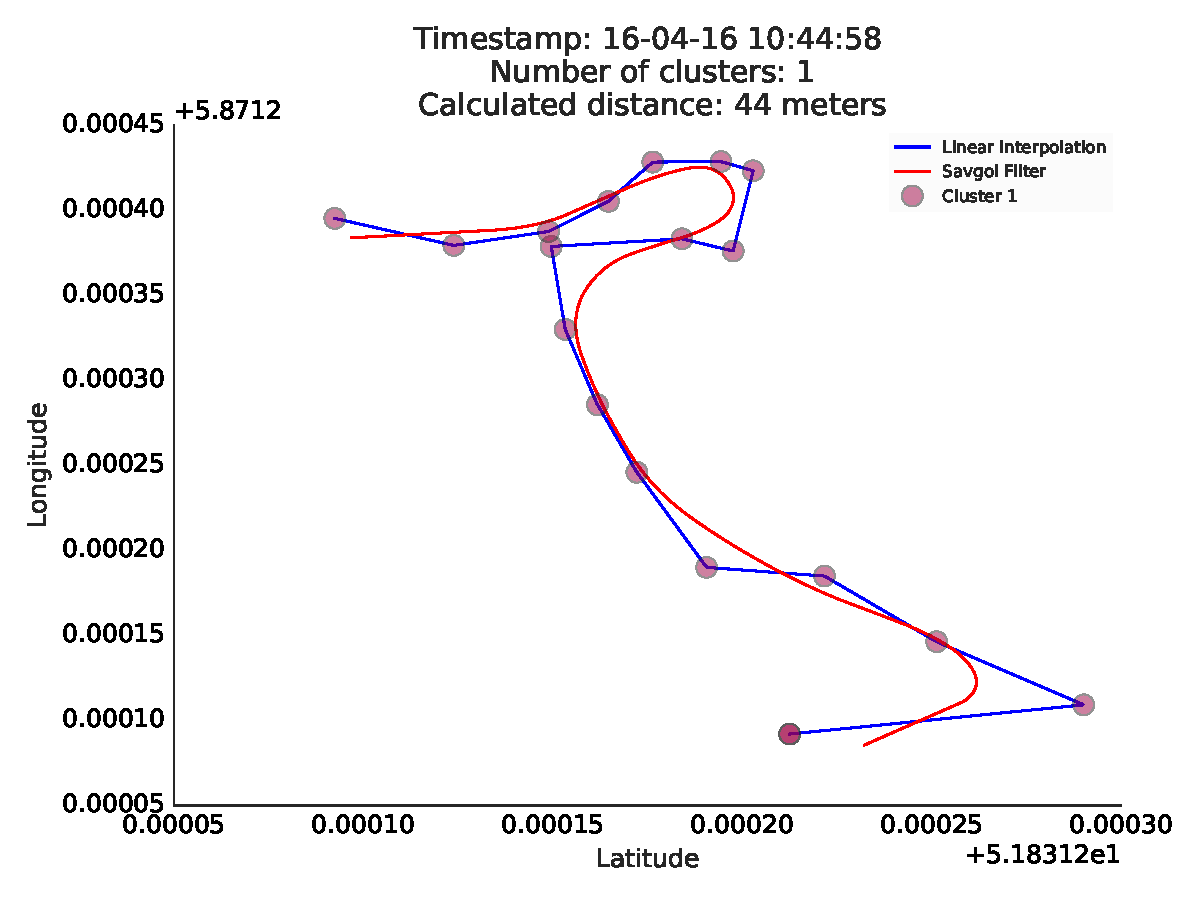
\includegraphics[scale=0.29]{gps/circle/4E2jhxMF392sEjWJF}
	}
	\vfill
	\subfloat[]{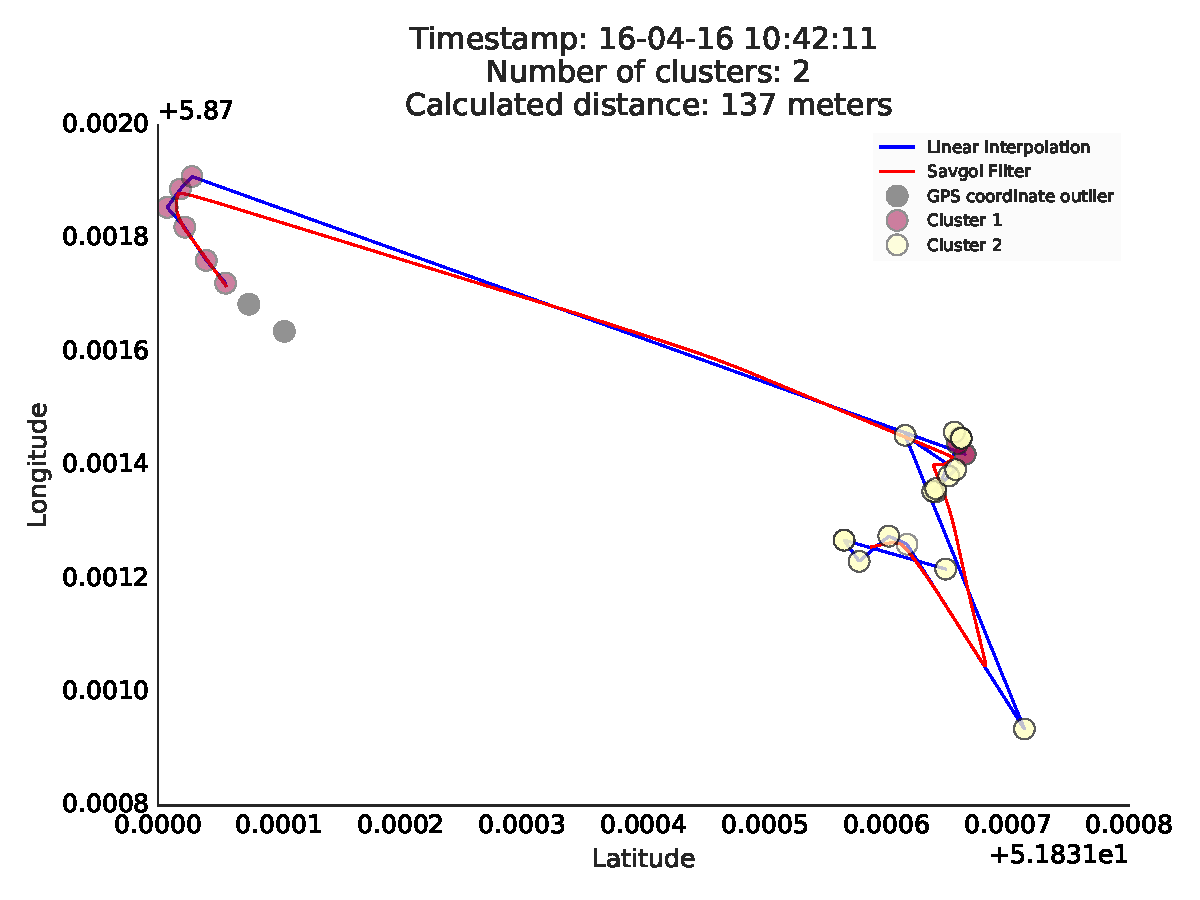
\includegraphics[scale=0.29]{gps/circle/HFgtoEcsXcmiDZHtY}
	}
	% Was eerst 141m door fout, nu 137
	\hspace{0.5cm}
	\subfloat[]{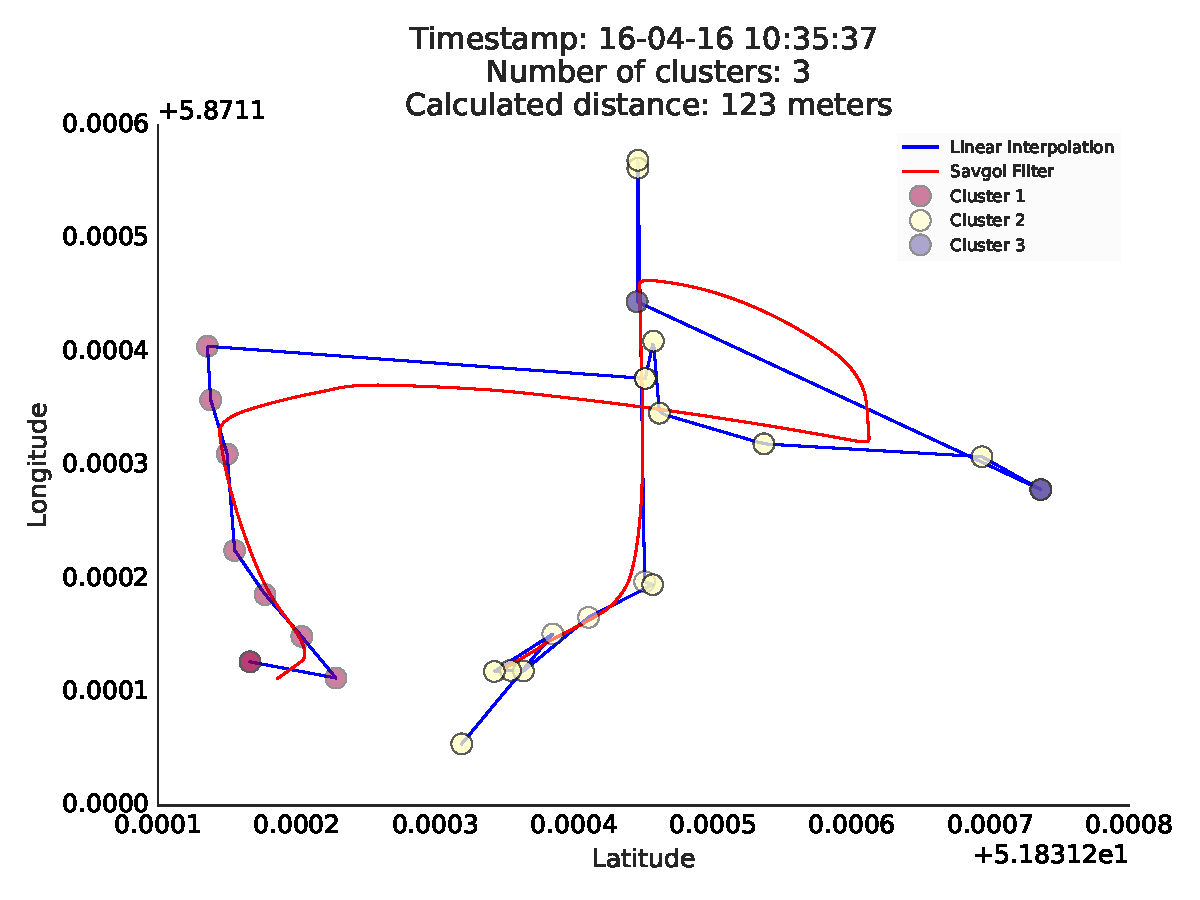
\includegraphics[scale=0.29]{gps/circle/otZE8i4oahYFNdegA}
	}
	\vfill
	\subfloat[]{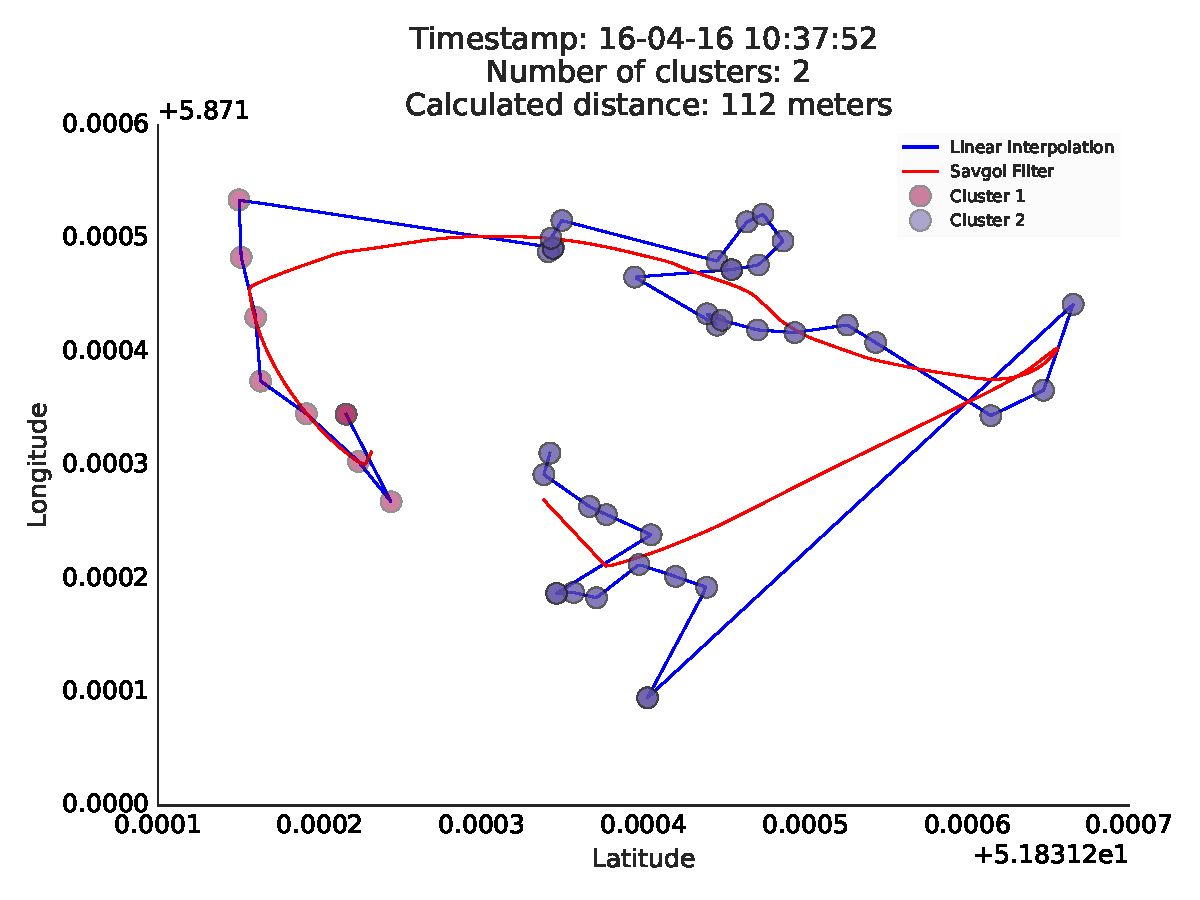
\includegraphics[scale=0.29]{gps/circle/Px5F2nQ9iaYACpJXG}
	}
	\captionof{figure}{Plots of the GPS coordinates of the walking test using a circular track. First, clustering is used to filter out the outliers. Afterwards, inliners are  smoothed in two stages: `Lineair Interpolation' is the first smoothing step and `Savgol Filter' the last. Black points are points classified as noise.}
\end{figure}

\newpage

\section{Heart Rate Boxplots}
\begin{figure}[H]
	\centering
	\subfloat[]{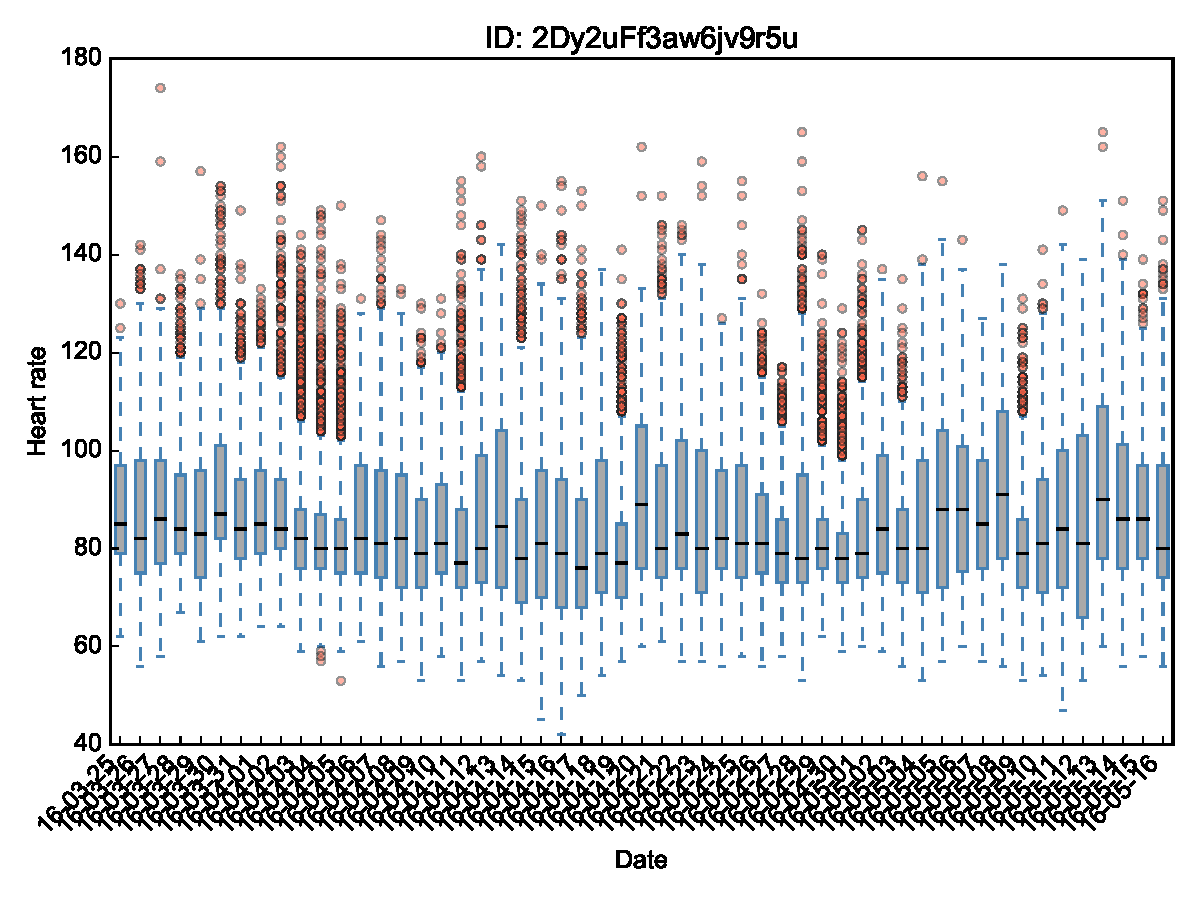
\includegraphics[scale=0.5]{boxplots/2Dy2uFf3aw6jv9r5u}
	}
	\vfill
	\subfloat[]{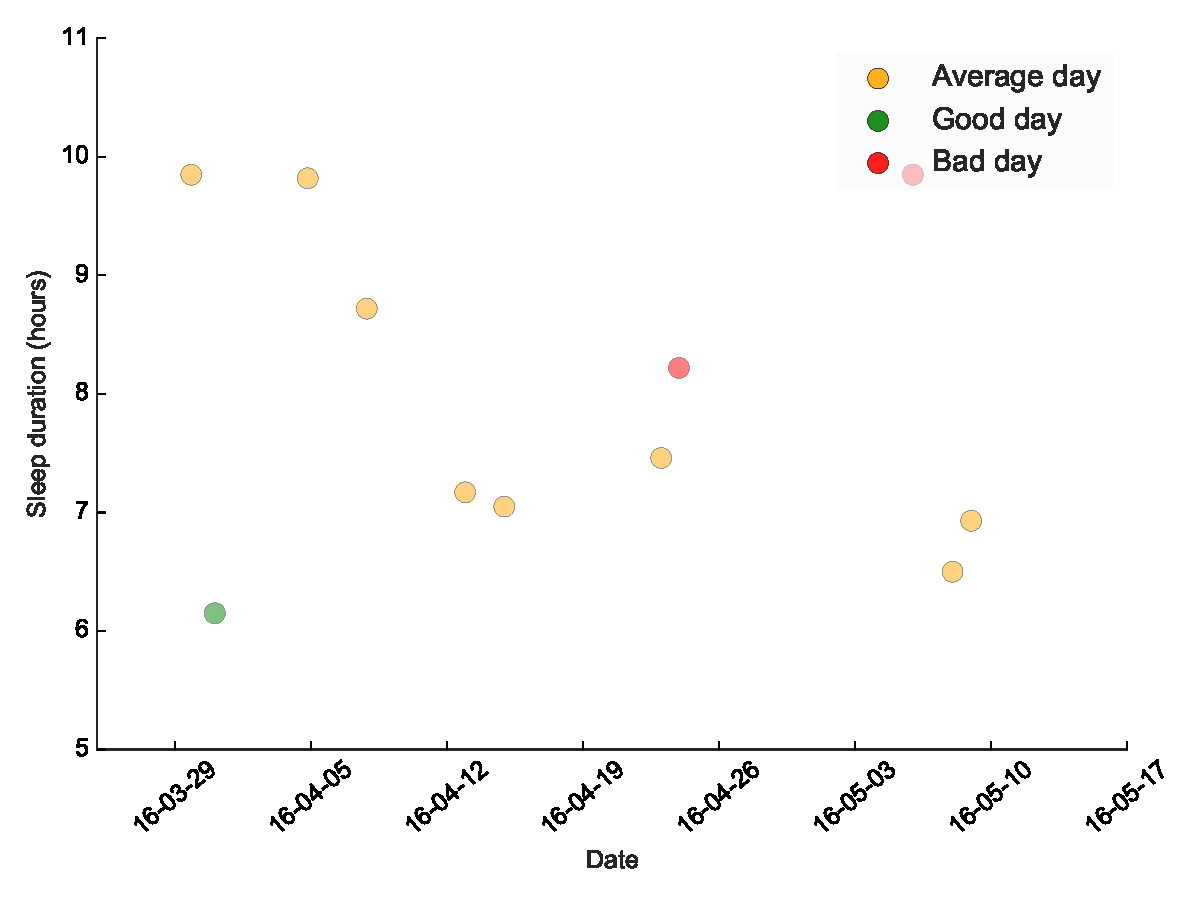
\includegraphics[scale=0.5]{boxplots/dW4YzJQEaidmyhsuY}
	}
	\captionof{figure}{Boxplots of the heart rates for each day.}
	\label{fig: heart rates boxplots}
\end{figure}

\begin{figure}
	\ContinuedFloat
	\centering
	\subfloat[]{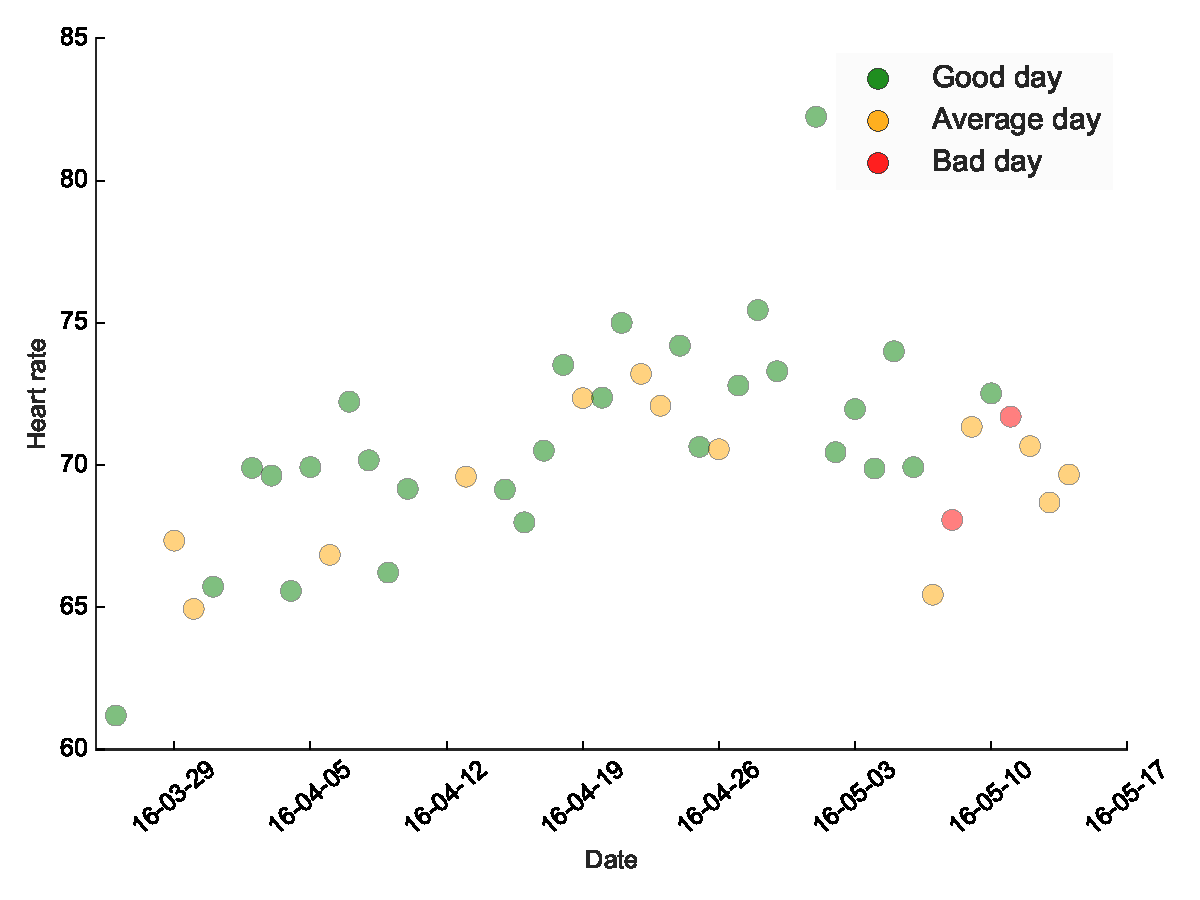
\includegraphics[scale=0.5]{boxplots/gGSWzh5PnqgFdCpq4}
	}
	\vfill
	\subfloat[]{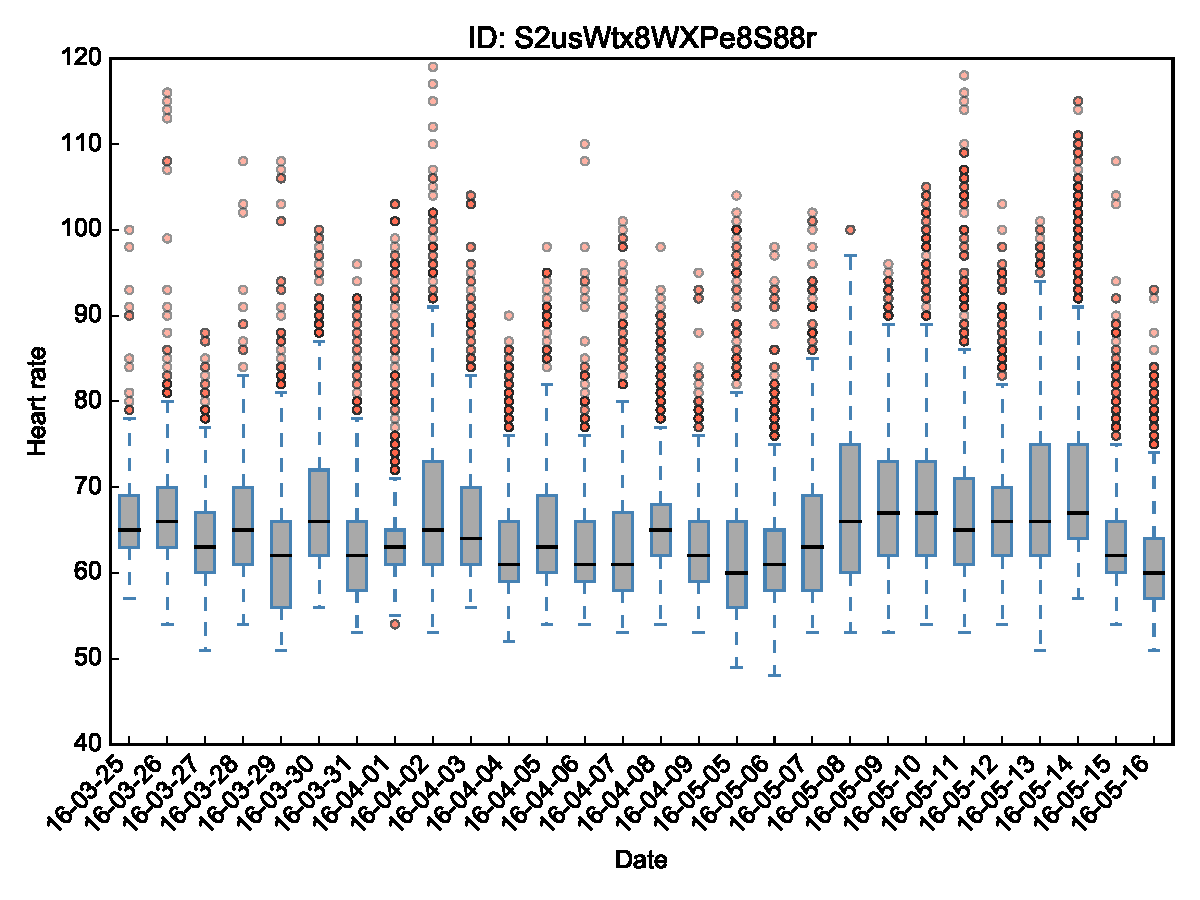
\includegraphics[scale=0.5]{boxplots/S2usWtx8WXPe8S88r}
	}
	\captionof{figure}{}
\end{figure}

\newpage

\section{Elliptic Outlier Detection}
%
\begin{code}
	\begin{minted}[linenos=true, fontsize=\footnotesize, breaklines=true]{python}
def PlotEllipticOutliers(rawPositions, ID, timestmp):
    """
    This method is used for outlier detection on a straight track.
    Uses the EllipticEnvelope object from Scikit-learn
    :param rawPositions:    The raw GPS positions
    :param ID:              The ID of the user
    :param timestmp:        The timestamp
    """
    folder = "out/"
    plotDir = folder + "plots/Walking Test"

    lats = []
    longs = []
    timestamps = []
    for pos in rawPositions:
        lat = pos["latitude"]
        long = pos["longitude"]
        timestamp = pos["timestamp"]
        lats.append(lat)
        longs.append(long)
        timestamps.append(timestamp)

    # writeToFile(ID, "output", lats, longs)
    classifiers = {
        "Robust Covariance Estimator": EllipticEnvelope(contamination=0.08, support_fraction=0.8)
    }
    alpha = 0.5
    linewidth = 0.15

    classifierName = "Robust Covariance Estimator"
    classifier = classifiers[classifierName]
    X = zip(lats, longs)
    xx1, yy1 = np.meshgrid(np.linspace(min(lats), max(lats), 1000), np.linspace(min(longs), max(longs), 1000))
    classifier.fit(X)
    Z1 = classifier.decision_function(np.c_[xx1.ravel(), yy1.ravel()])
    Z1 = Z1.reshape(xx1.shape)
    CS = plt.contour(xx1, yy1, Z1, levels=[0], linewidths=1, colors="g")
    CS.collections[0].set_label(classifierName)
    plt.scatter(lats, longs, s=50, alpha=alpha, linewidth=linewidth, edgecolor=almost_black, color="steelblue",
                label="GPS coordinate")
    plt.autoscale(enable=True, axis="both")
    filteredPositions = []

    for lat, long, timestamp in zip(lats, longs, timestamps):
        z = classifier.decision_function(np.c_[lat, long])
        if z > 0:  # Check if coordinate (lat, long) is within the ellipse
            filteredPositions.append((lat, long, timestamp))

    y = zip(*filteredPositions)[0]  # the latitudes
    x = zip(*filteredPositions)[1]  # the longitudes
    t = zip(*filteredPositions)[2]  # the timestamps

    x2, y2, newx2, newy2 = smooth(y, x, t)
    plt.plot(y2, x2, label="Linear Interpolation")
    totalDistance = calcDistanceWalked(newy2, newx2)

    plt.plot(newy2, newx2, label="Savgol Filter", color="r")
    plt.title("Timestamp: %s\n Calculated distance: %i meters" % (timestmp, totalDistance))
    plt.xlabel("Latitude")
    plt.ylabel("Longitude")
    fancyPlot()
    writeToPdf(ID, plotDir)

\end{minted}
	\caption{Code used for detecting outliers in a straight path.}
	\label{GPS Smoothing Code Straight Line}
\end{code}
%

\newpage

\section{Clustering Outlier Detection}
%
\begin{code}
	\begin{minted}[linenos=true, fontsize=\footnotesize, breaklines=true]{python}
def clustering(lats, longs, timestamps, ID, timestmp, multiPDF=False):
    """
    Clusters the GPS coordinates using DBSCAN
    :param timestmp:                The timestamp
    :param ID:                      The ID
    :param timestamps:              The timestamps of the GPS coordinates
    :param lats:                    The latitudes
    :param longs:                   The longitudes
    :return:                        The rounded distance
    """
    folder = "out/"
    plotDir = folder + "plots/Walking Test Analysis"

    R = 6371  # Radius of the earth in km
    cartesianX = []
    cartesianY = []
    cartesianZ = []

    for lat, long in zip(lats, longs):
        # Convert to cartesian coordinates
        x = R * cos(lat) * cos(long)
        y = R * cos(lat) * sin(long)
        z = R * sin(lat)
        cartesianX.append(x)
        cartesianY.append(y)
        cartesianZ.append(z)

    combined = np.vstack((cartesianX, cartesianY, cartesianZ)).T
    (core_samples, labels) = dbscan(combined, eps=0.5)
    grouped = zip(labels, core_samples)
    nonGroupedPositions = []

    for (label, core_sample) in grouped:
        if label != -1:
            lat = lats[core_sample]
            long = longs[core_sample]
            stamp = timestamps[core_sample]
            nonGroupedPositions.append((lat, long, stamp))

    if len(nonGroupedPositions) > 0:
        y = zip(*nonGroupedPositions)[0]  # the latitudes
        x = zip(*nonGroupedPositions)[1]  # the longitudes
        t = zip(*nonGroupedPositions)[2]  # the timestamps
        x2, y2, newx2, newy2 = smooth(y, x, t)

        plt.plot(y2, x2, label="Linear Interpolation")
        plt.plot(newy2, newx2, label="Savgol Filter", color="r")
        distance = calcDistanceWalked(newy2, newx2)
        grouped = sorted(grouped, key=itemgetter(0))

        clusters = {}
        labels = []
        for key, group in groupby(grouped, key=itemgetter(0)):
            # group the clusters based on their label
            labels.append(key)
            clusters[key] = [el[1] for el in group]

        noise = False
        colors = plt.get_cmap("Spectral")(np.linspace(0, 1, len(clusters)))
        for label in labels:
            indices = clusters[label]
            latitudes = []
            longitudes = []
            size = 10
            alpha = 0.5
            lineWidth = 0.15
            for i in indices:
                latitudes.append(lats[i])
                longitudes.append(longs[i])
            if label == -1:
                # outliers are identified with a label of -1
                plt.plot(latitudes, longitudes, "o", markerfacecolor=almost_black, markeredgecolor=almost_black,
                         markersize=size, alpha=alpha, linewidth=lineWidth, label="Outlier")
                noise = True
            else:
                plt.plot(latitudes, longitudes, "o", markerfacecolor=colors[label], markeredgecolor=almost_black,
                         markersize=size, alpha=alpha, linewidth=lineWidth, label="Cluster %i" % (label + 1))

        plt.title("Timestamp: %s\n Number of clusters: %i\n Calculated distance: %i meters" % (
            timestmp, (len(clusters) - 1) if noise else len(clusters), round(distance)))
        plt.xlabel("Latitude")
        plt.ylabel("Longitude")
        fancyPlot()
        writeToPdf(ID, plotDir)
        return True, distance
    else:
        # DBSCAN gave back an empty array, therefore we cannot perform any smoothing or distance calculation
        return False, 0
\end{minted}
	\caption{Code used for detecting outliers in a non-straight path.}
	\label{GPS Smoothing Code Non-Straight Line}
\end{code}
%

\newpage

\section{Calculation of Walking Speed}
%
\begin{code}
	\input{code/"Walking speed".tex}
	\caption{Code used for calculating the walking speed between GPS coordinates.}
	\label{walk test code snippet}
\end{code}
%


\section{Tables}
\subsection{Sleep}
% !TeX spellcheck = en_US
% !TeX root = ../BachelorThesis.tex

\begin{table}[H]
 	\centering
 	\begingroup
 	\fontsize{6pt}{6pt}
 	\selectfont
 	\subfloat[]{
 		\csvautobooktabular[head to column names, table head=\toprule \bfseries Date & \bfseries Rating & \bfseries Duration (h)\\\midrule]
 		{csv/sleep/2Dy2uFf3aw6jv9r5u.csv}
 		\label{table:sleepduration1}
 	}
 	\hspace{1cm}
 	\subfloat[]{
 		\csvautobooktabular[head to column names, table head=\toprule \bfseries Date & \bfseries Rating & \bfseries Duration (h)\\\midrule]
 		{csv/sleep/dW4YzJQEaidmyhsuY.csv}
 		\label{table:sleepduration2}
 	}
 	\captionof{table}{Measurements of the sleep duration of our participants.} 
	\label{table: Sleep Analysis}
	
	\endgroup
\end{table}

\begin{table}[H]
	\ContinuedFloat
	\centering
 	\begingroup
 	\fontsize{6pt}{6pt}
 	\selectfont
 	\subfloat[]{
 		\csvautobooktabular[head to column names, table head=\toprule \bfseries Date & \bfseries Rating & \bfseries Duration (h)\\\midrule]
 		{csv/sleep/gGSWzh5PnqgFdCpq4.csv}
 		\label{table:sleepduration3}
 	}
 	\hspace{1cm}
 	\subfloat[]{
 		\csvautobooktabular[head to column names, table head=\toprule \bfseries Date & \bfseries Rating & \bfseries Duration (h)\\\midrule]
 		{csv/sleep/S2usWtx8WXPe8S88r.csv}
 		\label{table:sleepduration4}
 	}
 	\captionof{table}{}
	\endgroup
\end{table}
\subsection{Heart Rate}
\input{tables/"heart rate"}
\subsection{Walking Test}
\input{tables/"walking test"}


